% !TEX program = xelatex
% 第一轮只编译本模板；生成结果后，以下三个输入自动替换占位说明。
% 使用 TeX Live 自带的 Fandol 字体，不依赖某一台电脑的专有字体。
\documentclass[UTF8,fontset=fandol,11pt,a4paper]{ctexart}
\usepackage[margin=2cm]{geometry}
\usepackage{amsmath,booktabs,graphicx}
\setlength{\parindent}{0pt}
\setlength{\parskip}{0.35em}
\pagestyle{empty}

\begin{document}
\begin{center}
  {\Large 蒲丰投针：从模拟到报告}\\[0.3em]
  {\small W3 数值实验}
\end{center}

\section*{实验目的与方法}
用随机投针的相交比例估计圆周率。针长不大于平行线间距；针位和角度独立均匀取样。
记投针数为 $N$、相交数为 $K$、针长为 $L$、线间距为 $d$，当 $K>0$ 时使用
$\widehat{\pi}=2LN/(dK)$。

\IfFileExists{results-params.tex}{
  本次实验使用 seed $=$ 42，针长 $L=0.5$，平行线间距 $d=1$；共 3 组投针，投针数 $N=1000, 10000, 100000$。

}{
  \textit{参数尚未生成。运行实验和图表程序后，这里将显示实际 seed、投针数、针长和线间距。}
}

\section*{实验结果}
\begin{center}
\IfFileExists{results-table.tex}{
  \begin{tabular}{rrr}
\toprule
投针数 $n$ & 相交数 $K$ & 估计值 $\widehat{\pi}$ \\
\midrule
1000 & 305 & 3.278689 \\
10000 & 3198 & 3.126954 \\
100000 & 31921 & 3.132734 \\
\bottomrule
\end{tabular}

}{
  \fbox{\parbox{0.85\linewidth}{\centering 表格尚未生成。这是模板首次编译时的正常状态。}}
}
\end{center}

\begin{center}
\IfFileExists{results.png}{
  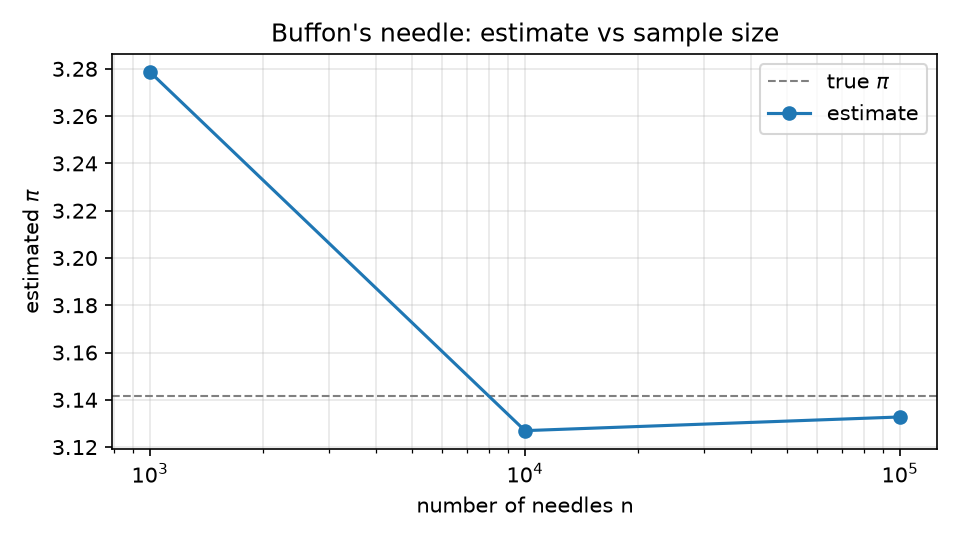
\includegraphics[width=0.85\linewidth,height=0.28\textheight,keepaspectratio]{results.png}
}{
  \fbox{\parbox[c][3cm][c]{0.85\linewidth}{\centering 图像尚未生成。图表程序必须读取真实的 results.csv。}}
}
\end{center}

\section*{一条观察}
本次三组估计值分别为 $3.2787$、$3.1270$、$3.1327$，都落在真值 $\pi$ 附近；
对应的相交比例为 $305/1000$、$3198/10000$、$31921/100000$，接近理论值
$2L/(\pi d)=1/\pi\approx0.3183$。这里不把“样本越大误差必减”当作判据：
从 $N=1000$ 到 $10000$ 明显更接近，而 $10000$ 到 $100000$ 变化很小；
估计值只由本次实际相交数决定，不保证逐次逼近。

\end{document}
